\renewcommand{\tablename}{\textbf{Tabla}}

En este capítulo de la tésis se describe detalladamente la plataforma de fuente abierta que desarrollamos para renovar la electrónica y el \textit{software} de control del espectrofluorímetro Horiba PTI Quanta Master (QM 400), uno de los espectrofluorímetros antigüos del laboratorio de fotoquímica del INQUIMAE.
Además de su renovación, ampliamos sus capacidades para medir tiempos de vida del orden de los microsegundos, que junto con el agregado de un láser pulsado externo de 980 nm nos permitió conseguir la plataforma ideal para la caracterización óptica de UCNPs tanto estática como dinámica.


\section{Renovación y ampliación del fluorímetro Horiba PTI Quanta Master 400}

\subsection{Componentes originales}

La serie Horiba PTI QM incluye espectrofluorímetros modulares para investigación científica y sistemas optimizados para mediciones de fotoluminiscencia.
Estos espectrofluorímetros se encuentran frecuentemente en los laboratorios de Argentina, por ejemplo, sabemos que hay tres equipos de esta serie en el laboratorio de fotoquímica del INQUIMAE (QM400, QM-4 y RatioMaster), dos en el Centro de Investigaciones en Bionanociencias (CIBION) y uno en el Centro Atómico Constituyentes de la Comisión Nacional de Energía Atómica (CAC-CNEA), y probablemente haya más similares en otras instituciones.
Al ser modelos antigüos y descontinuados se pueden encontrar en el mercado por precios que rondan los \$5000 USD, un costo relativamente bajo para un espectrofluorímetro científico.
Los bajos costos se dan por su antigüedad y fin de soporte por parte de la empresa, lo que obliga a los usuarios a resolver ellos mismos los problemas que haya con los equipos.
Por ejemplo, en CIBION, uno de los dos modelos que tienen no está funcionando porque hay problemas con la inicialización de los controladores en la PC.
En este trabajo, reacondicionamos específicamente un espectrofluorímetro QM 400 de más de 30 años de antigüedad,  (diagrama en la \textbf{Fig. \ref{fig:ref-diagram}A} y fotografía en la \textbf{Fig. \ref{fig:hardware}A}), pero dada la similitud entre los distintos modelos de esta serie, la renovación se pueden aplicar a cualquiera de ellos con leves modificaciones. 

El QM 400 está equipado con una lámpara de xenón de 75 W como fuente de luz, la cual proporciona un amplio espectro de longitudes de onda (desde el infrarrojo cercano, alrededor de 1000 nm, hasta el ultravioleta, alrededor de 300 nm).
Los monocromadores de excitación y emisión contienen redes de difracción rotadas por motores paso a paso de 200 pasos por revolución, con especificaciones de 7 V y 0.7 A por bobina (M1 y M2), lo que permite una resolución en la selección de longitudes de onda de 0.5 nm. 
Ambos incluyen un fin de carrera electromecánico para verificar si se ha alcanzado la longitud de onda máxima.
Los motores paso a paso, junto con sus fines de carrera respectivos, están conectados a un módulo controlador de motores (MDM) mediante conectores propietarios no documentados. 
Los fotones son detectados por un tubo fotomultiplicador (PMT, modelo PTI 810), cuya caracterización se detalla en la sección \ref{sec:caracterizacion_pmt}.
Éste está conectado al MDM a través de un cable BNC y polarizado con 1000 V desde una fuente de alimentación externa proporcionada también por el MDM. 
Esto genera pulsos eléctricos ante la llegada de cada fotón al detector (\textbf{Fig. \ref{fig:ref-diagram}D}). 
Finalmente, el MDM está conectado mediante un cable plano a una tarjeta de interfaz ISA en una PC con sistema operativo Windows 95 y el programa FelixGX, un \textit{software} propietario de adquisición y control instalado por Horiba (\textbf{Fig. \ref{fig:ref-diagram}B}).
FelixGX permite medir espectros de emisión y excitación (\textbf{Fig. \ref{fig:ref-diagram}E}), además de brindar herramientas de análisis rápido de los datos y controlar diferentes periféricos.

La antigüedad de la PC y electrónica de control hace que el proceso de adquisición de datos sea tedioso, y más aún para la caracterización de UCNPs.
Para hacer una medición el usuario debe colocar la muestra en la cámara y luego configurar en FelixGX un barrido de la longitud de onda de excitación o emisión.
La única forma de extraer los datos es a través de un disquette, ya que la PC tampoco cuenta con conexión a la red.
En el caso de medir \textit{upconversion} se debe agregar un láser controlado externamente por una fuente de corriente (\textbf{Fig. \ref{fig:ref-diagram}A}) en la que se debe configurar por separado los parámetros de excitación, como la potencia.
Una plataforma de caracterización óptica completa de UCNPs debería ser capaz de medir espectros de emisión y tiempos de vida (del orden de los microsegundos) excitando a 980 nm con distintas densidades de potencia.
Además, como las mediciones de espectro y tiempo de vida son de larga duración (en especial a bajas potencias), resulta ideal que la plataforma permita configurar múltiples mediciones sucesivas sin la necesidad de una configuración manual por el usuario.
Durante su tésis de doctorado, Juan Bujjamer agregó la capacidad de medir tiempos de vida típicos de \textit{upconversion} al QM 400 \cite{bujjamer2020}. 
Para lograrlo utilizó en conjunto el control de los monocromadores que brinda FelixGX, una CPU y FPGA Red Pitaya y una fuente de diodo láser externa.
El excelente trabajo de Juan sentó las bases para que en este trabajo podamos hacer una renovación total del QM 400, utilizando como única plataforma de control a la Red Pitaya e independizandonos de la PC de control original.
En las siguientes secciones, explicaremos los cambios de \textit{hardware} y \textit{software} que realizamos en el espectrofluorímetro para que sea una plataforma ideal para medir \textit{upconversion}.



\begin{figure}[btp]
     \centering
     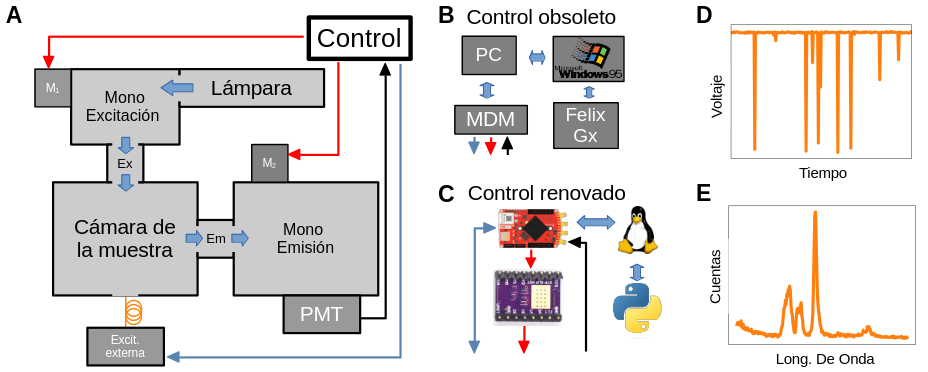
\includegraphics[width=\textwidth]{spec_diagram.png}
     \caption{
     \textbf{Representación esquemática del espectrofluorímetro}
     (\textbf{A}) Diagrama del hardware del Horiba PTI QM 400. Las flechas rojas representan los conectores de motores y fines de carrera, las negras corresponden a BNC, las azules a USB y las naranjas representan fibra óptica. La trayectoria de la luz dentro del espectrómetro está indicada con flechas azules gruesas.
     (\textbf{B}) y (\textbf{C}) Representación del módulo de control instrumental antiguo y nuevo, respectivamente.
     (\textbf{D}) Representación de la señal cruda medida por el detector PMT.
     (\textbf{E}) Espectro de la muestra construido a partir del conteo de picos en las señales crudas medidas para cada longitud de onda.
    }
     \label{fig:ref-diagram}
\end{figure}

\begin{figure}[h]
     \centering
     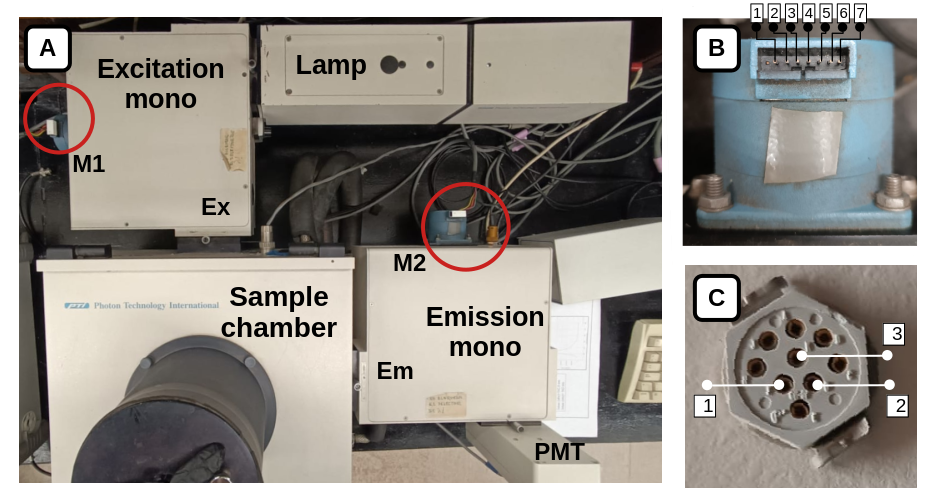
\includegraphics[width=0.9\textwidth]{hardware.png}
     \caption{\textbf{Foto del Horiba PTI Quanta Master 400}. 
    (\textbf{A}) Imagen del espectrómetro completo. En rojo se señalan los motores de los monocromadores y los fines de carrera. (\textbf{B}) Diagrama de pines de los motores paso a paso. Los únicos pines utilizados en la versión renovada son 1 y 7, y 3 y 5, que corresponden a cada bobina del motor respectivamente. (\textbf{C}) Diagrama de pines de los fines de carrera. Los únicos utilizados son los señalados en la imagen.}
     \label{fig:hardware}
\end{figure}


\subsection{Hardware para la renovación del QM 400}

Luego de hacer una inspección de todas las partes, decidimos conservar los componentes ópticos, la motorización, el PMT, la fuente de alta tensión y el chasis, ya que son robustos y funcionales.  
En contraste, la electrónica de control y detección resultó ser voluminosa, de código cerrado y obsoleta, por lo que optamos por reemplazarla con alternativas modernas: una CPU con FPGA integrada Red Pitaya (RP) STEM LAB 125-14.
La RP cuenta con cuatro entradas y salidas analógicas que emiten y procesan señales en las radiofrecuencias, y un conjunto de pines digitales que permiten controlar circuitos integrados fácilmente.
Esta placa junto con dos circuitos integrados DRV8825 que simplifican el control de los motores por paso cumplen la tarea de controlar a los monocromadores.
Este cambio en la electrónica de control nos permitió reemplazar el voluminoso módulo MDM ($\sim$10 cm $\times$ 30 cm $\times$ 30 cm) por dos controladores DRV8825 soldados a una placa PCB mucho más pequeña (10 cm$\times$ 10 cm $\times$ 2 cm)(\textbf{Fig. \ref{fig:placa}}).

Para facilitar la conexión de los componentes del espectrofluorímetro a la RP también agregamos a la placa un puerto IDC que permite conectar los pines digitales, y conectores a los motores a través de fichas adaptadas a medida.
Tanto el diseño de los conectores a los motores como el de los fines de carrera son de propietario y no están estandarizados ni documentados.
Por este motivo, tuvimos que comprar fichas estandarizadas en el mercado y adaptarlas a mano para que encajaran.
La conexión a los fines de carrera fue particularmente difícil de llevar a cabo (\textbf{Fig. \ref{fig:hardware}C}).
Estos conectores consisten de nueve pines, pero no hay ningún manual técnico del instrumento que especifique cuáles son las conexiones a cada uno.
Para averiguarlo, tuvimos que conectar un osciloscopio entre cada pin y el MDM original, y al mismo tiempo mover los motores cruzando el límite de longitud de onda para ver cómo era la señal.
Finalmente llegamos a la conlcusión de que sólo tres de los nueve pines se utilizan. 
Dos pines son de alimentación entre 0 y 5 V, y el tercero es una señal TTL que indica si el monocromador se pasó del límite o no.
Nuestra solución -temporaria para avanzar mientras conseguimos los conectores correctos- para hacer la conexión consistió en soldar cables de red con las puntas peladas a la PCB y conectarlos en los orificios del fin de carrera.
Por último, el PMT se conecta a través de un cable BNC-SMA a uno de los canales analógicos de radiofrecuencias de la RP, luego son digitalizados por su conversor analógico digital (ADC)(\textbf{Fig. \ref{fig:ref-diagram}D}) de 14 bits y luego contados por software (\textbf{Fig. \ref{fig:ref-diagram}E}).
Todas las conexiones se ven detalladas en la figura (\textbf{\ref{fig:connection_diagram}}).

La RP tiene una interfaz de programación de aplicaciones (API) que permite configurar dos métodos distintos para comenzar una adquisición de datos.
Una opción es llamar a una función que comienza la adquisición de inmediato.
Alternativamente, se puede configurar una de las entradas analógicas o digitales como \textit{trigger} para comenzar una medición.
Nosotros usamos el primer método para medir espectros estáticos y el otro para medir tiempos de vida.
Asimismo, la RP tiene dos mecanismos distintos para escribir los datos en la memoria al hacer una adquisición: un método por defecto de escritura a un espacio de memoria de 2$^{14}$ enteros de 16 bits, y un método de adquisición de memoria profunda (DMA) que permite guardar hasta 2 MB \cite{DMA_rp}.
Con esta capacidad para almacenar datos, a 31.25 MHz la ventana temporal de pulsos más grande que se puede obtener es de $\sim 0.5$ ms y $\sim 8$ ms respectivamente.
Aunque resulta beneficioso el método DMA y se podría implementar en esta renovación, nosotros utilizamos el método por defecto por la simplicidad que significó durante el desarrollo.
Para contrarrestar la corta duración de la ventana de adquisición, el software de control que desarrollamos permite agregar una demora para obtener ventanas de medición más grandes (ver sección \ref{sec:proceso_dinamico}).
El apéndice (\textbf{\ref{apendice:instrucciones_armado}}) explica detalladamente cómo reproducir las conexiones.

\begin{figure}
     \centering
     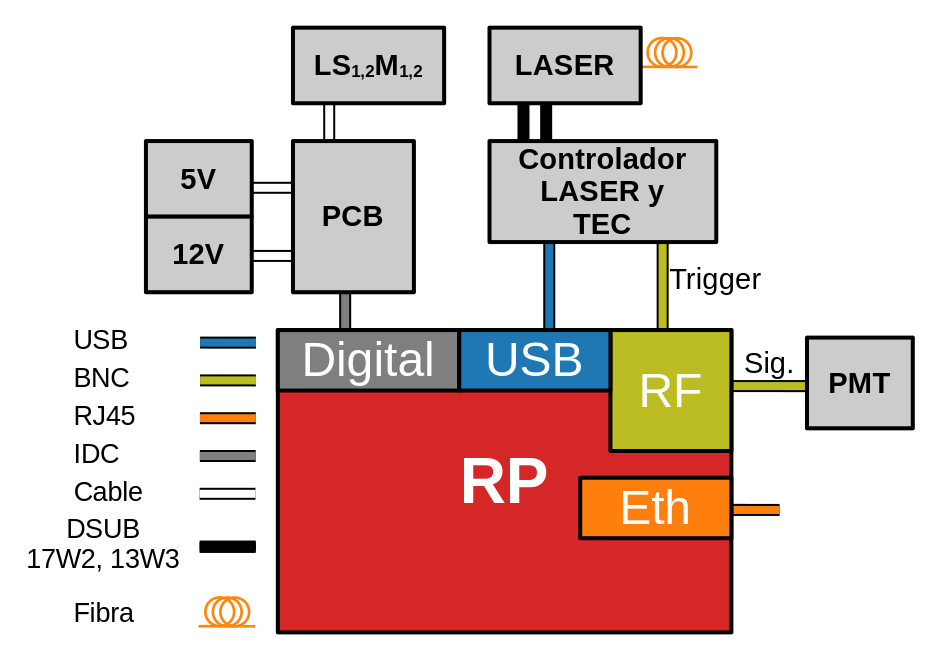
\includegraphics[width=0.8\textwidth]{connection_diagram.png}
     \caption{
    \textbf{Conexiones necesarias para la renovación y ampliación del QM400.}
    }
     \label{fig:connection_diagram}
\end{figure}



\subsection{Hardware para la medición de tiempos de vida}

El espectrofluorímetro original QM 400 disponible en el laboratorio no era adecuado para estudiar \textit{upconversion}, ya que no contaba con una fuente de luz en el infrarrojo (IR). 
Tampoco era posible realizar mediciones de tiempos de vida de la luminiscencia debido a la falta de excitación pulsada y detección dependiente del tiempo. 
Luego de aplicar renovación mencionada anteriormente, incorporamos estas funcionalidades al equipo y al \textit{software} de forma independiente.

Para ello, añadimos una fuente de luz IR externa modulable al sistema. 
En nuestro caso, utilizamos un controlador de diodo láser y temperatura (TEC) de banco THORLABS ITC4020, controlado por la RP, para operar un diodo láser BL976-SAG300 de 976 nm y 300 mW. 
La salida del diodo láser se conecta mediante una fibra óptica a la entrada de fuente externa del QM 400 (\textbf{Fig. \ref{fig:ref-diagram}A}). 
El ITC4020 permite configurar la frecuencia de pulsado y el ciclo de trabajo, además de proporcionar una señal TTL que está en 5 V cuando el láser está prendido y 0 V cuando está apagado.
Esta señal se conecta a otra de las entradas analógicas de la RP, que luego la utiliza como \textit{trigger} para sincronizar la finalización de la excitación del láser, con la medición de los pulsos eléctricos de los fotones.
Esa sincronización le permite al \textit{software} realizar histogramas y así medir los tiempos de vida, proceso que se explica en detalle en la sección \ref{sec:proceso_dinamico}.  


\begin{figure}[h]
     \centering
     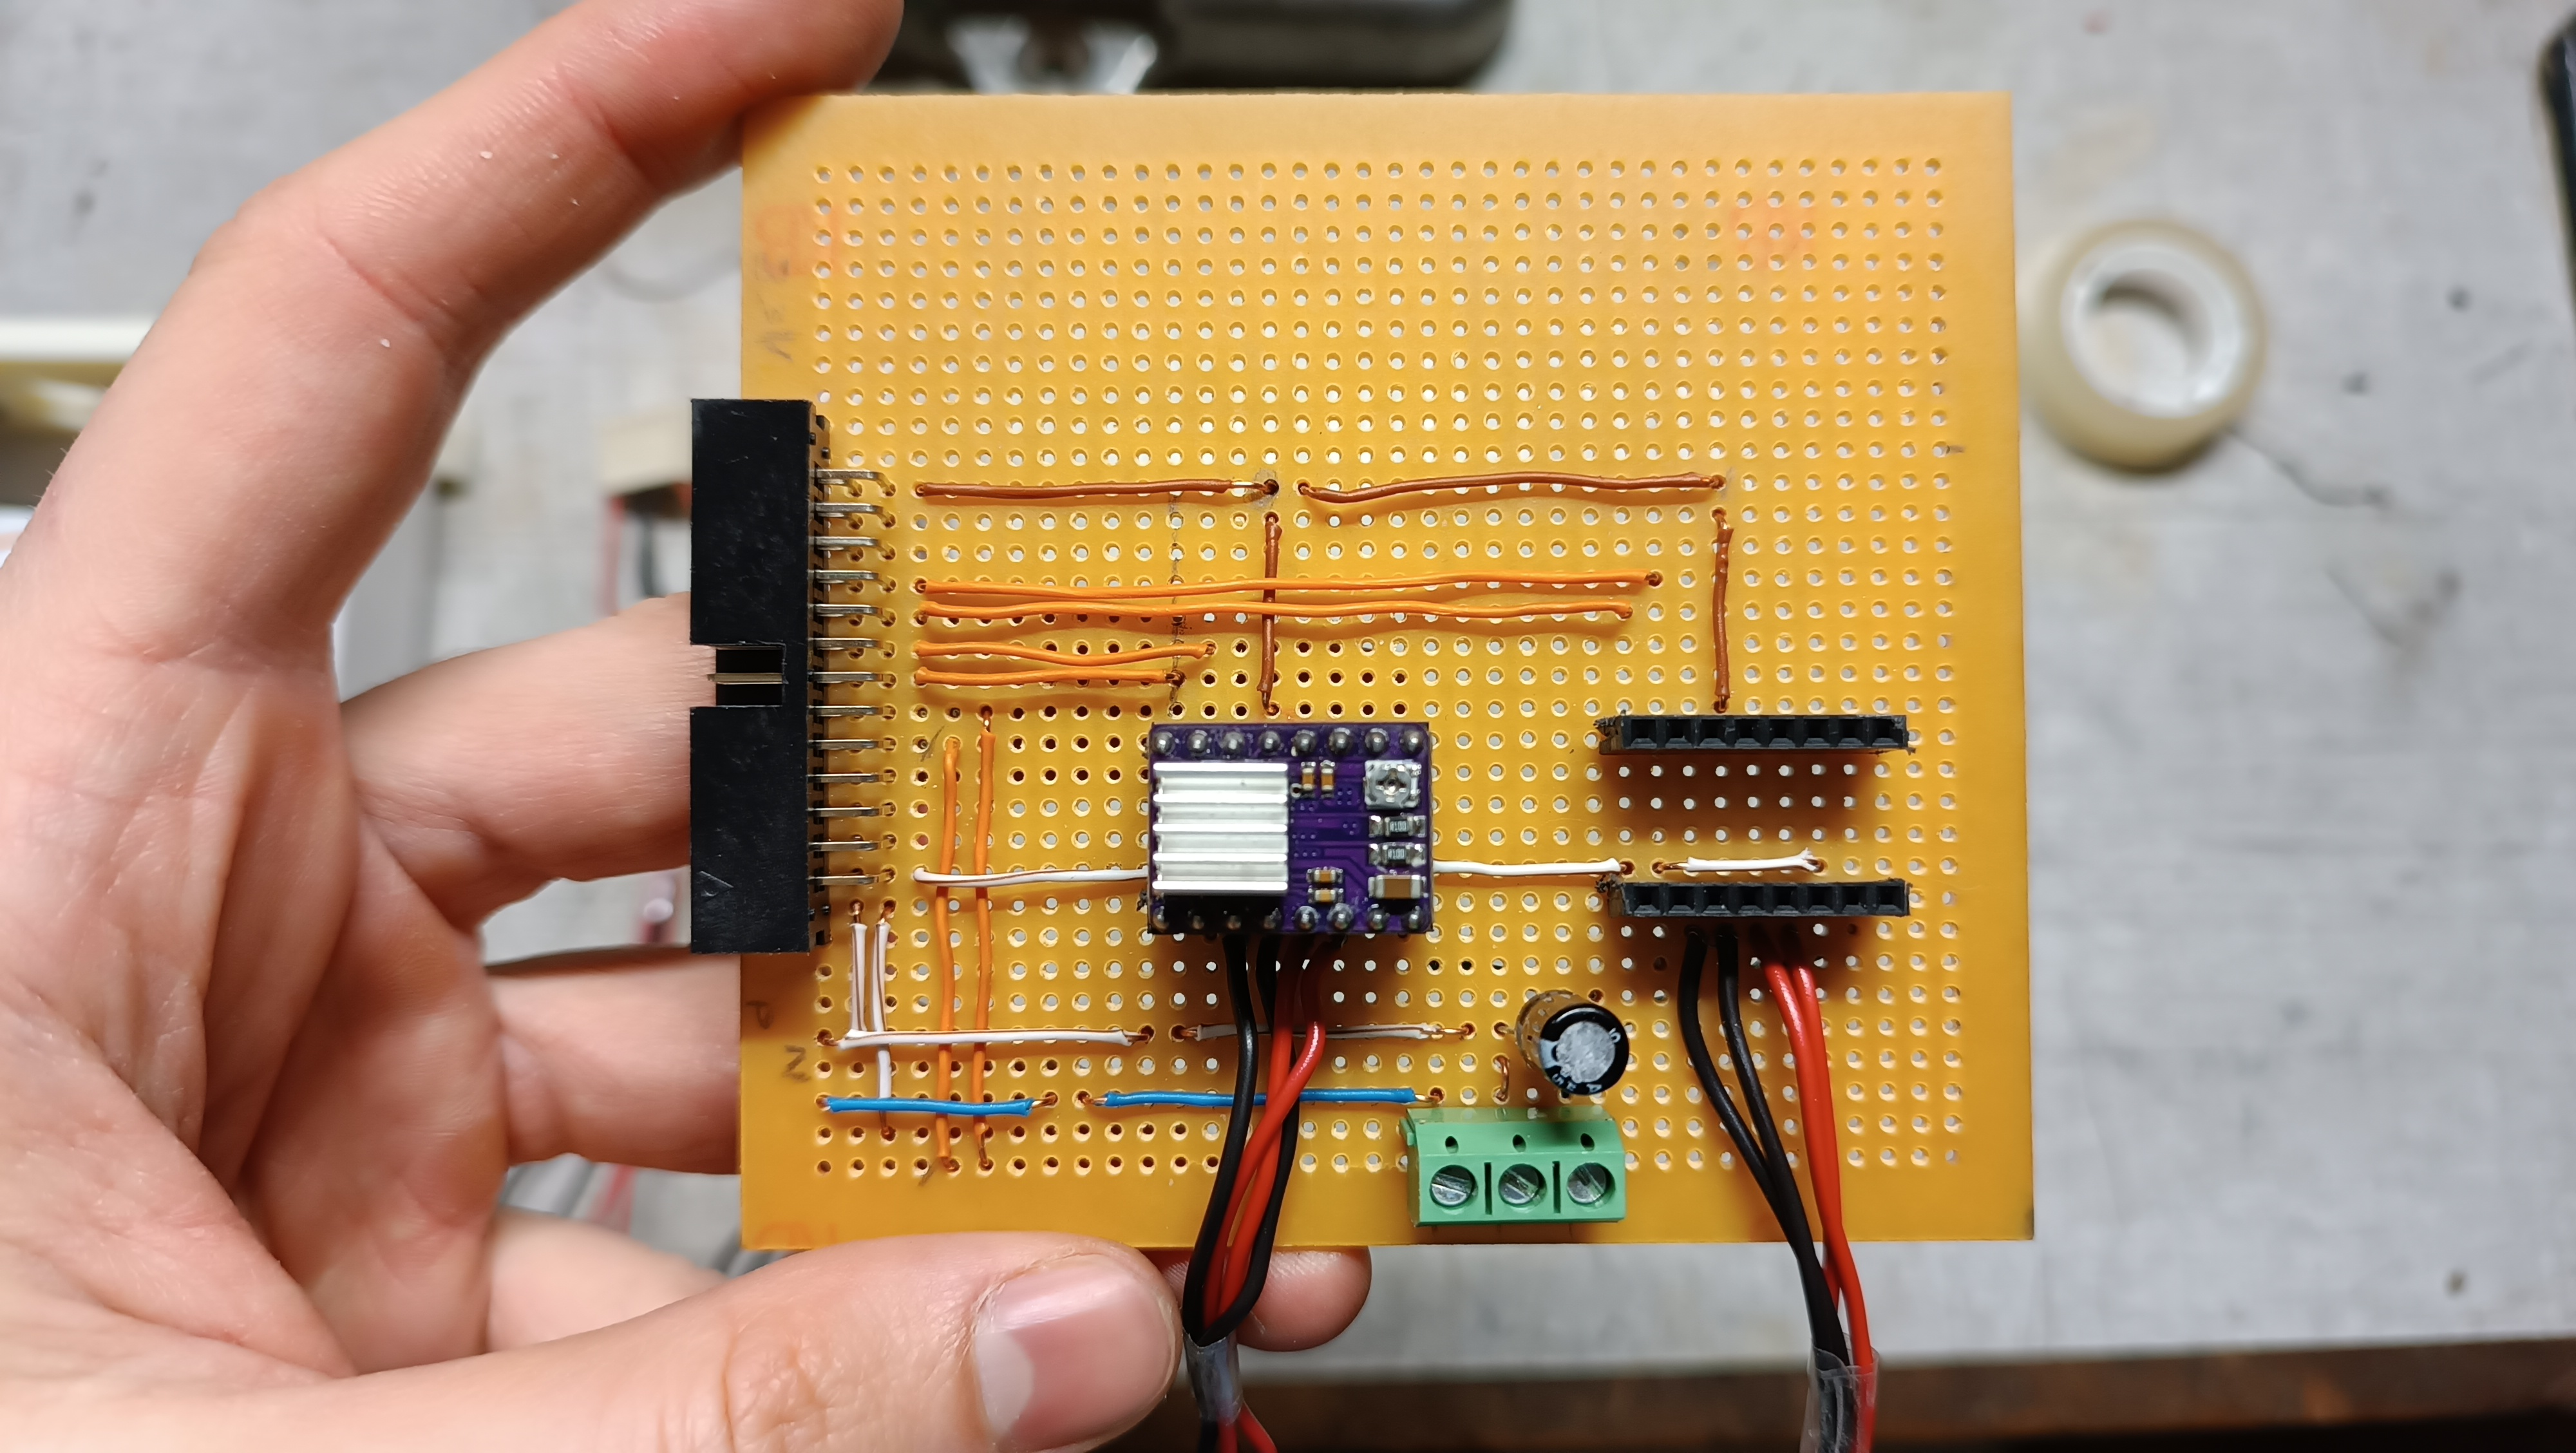
\includegraphics[width=0.9\textwidth]{placa.jpg}
     \caption{\textbf{Placa PCB con la electrónica de control.} La placa cuenta con un puerto IDC (izquierda) al que se conectan los pines digitales de la RP, que además provee la alimentación de 3.3 V a los circuitos integrados (centro). La placa incluye una bornera para proveer una referencia a tierra, una alimentación de 5 V y otra de 12 V.}
     \label{fig:placa}
\end{figure}


\section{Sistema de detección de fotones}


 
Los tubos fotomultiplicadores (PMTs) son detectores de fotones ampliamente utilizados en fluorómetros y cumplen un rol central en el funcionamiento del instrumento. 
Un PMT está compuesto por un fotocátodo y una serie de dínodos, que actúan como etapas de amplificación. 
Los fotones incidentes provocan la emisión de electrones desde el fotocátodo, y estos son amplificados sucesivamente por los dínodos. 
Al final del proceso, que tiene una duración típica de 40 a 50 nanosegundos, el pulso llega a un ánodo, desde donde se lee la señal \cite{lakowicz_principles_2006}. 
Este detector puede operar en dos modos: analógico o conteo de fotones. 
En el modo analógico, la corriente que fluye por el ánodo debe ser proporcional a la intensidad de luz que incide sobre el fotocátodo.
En el modo de conteo, el PMT registra pulsos eléctricos de corta duración cada vez que se detecta un fotón. 
Resulta crucial que el detector no se encuentre dañado, cosa que usualmente sucede por la exposición a luz muy intensa. 
Esto puede generar una corriente de oscuridad alta, pulsos espurios en la señal que sesgan el resultado de la medición \cite{lakowicz_principles_2006}.
En nuestro instrumento renovado, la señal del PMT se adquiere utilizando una Red Pitaya (RP). 
Este dispositivo permite una frecuencia máxima de adquisición de 125 MHz, aunque también es posible trabajar a frecuencias menores que sean divisiones por 2 de ese valor. 
Para realizar un conteo preciso de los fotones que inciden en el fotocátodo, caracterizamos la señal del PMT del QM 400 utilizando la RP en las mismas condiciones operativas del fluorímetro modificado.
Como resultado, medimos la corriente de oscuridad, determinamos el ancho medio de los pulsos y definimos el algoritmo de detección de pulsos más adecuado para optimizar el conteo. 
En las próximas secciones describimos en detalle esta caracterización.



\subsection{Caracterización del PMT con la Red Pitaya} \label{sec:caracterizacion_pmt}

\begin{figure}
    \centering
    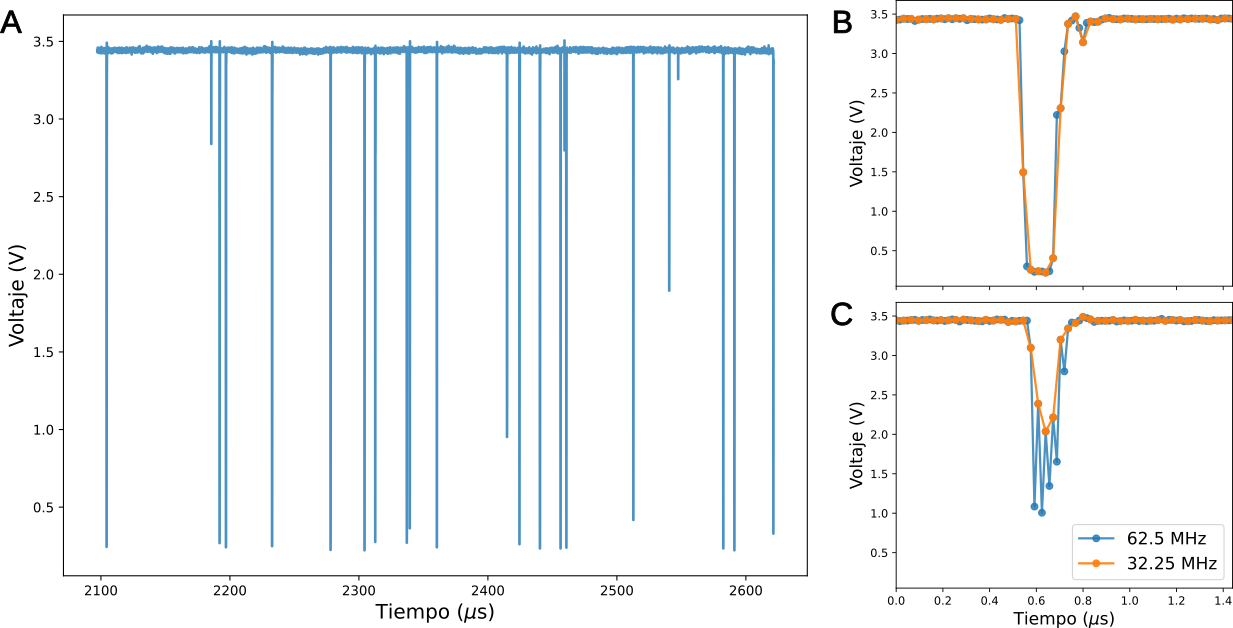
\includegraphics[width=\textwidth]{sig_pmt.png}
    \caption{\textbf{Señal del PMT.} (\textbf{A}) Medición de la señal del PMT en una ventana de la RP. Medidos a 62.5 MHz (azul) y 31.25 MHz (naranja): (\textbf{B}) detalle de un pulso que satura al PMT, (\textbf{C}) Detalle de un pulso que no satura el PMT.}
    \label{fig:pmt_signal}
\end{figure}

Una señal típica del PMT al ser iluminado de forma constante, medida con una ventana de la RP a 31.25 MHz,  se puede ver en la figura (\textbf{\ref{fig:pmt_signal}A}).
La señal muestra un voltaje de base que ronda los 3.5 V, y múltiples picos negativos que representan la llegada de un fotón al fotocátodo.
Si bien la mayoría de pulsos suelen estar entre 1 y 0 V, hay otros que no llegan a saturar el detector y tienen menor altura.
Los pulsos que saturan tienen un tiempo rápido de subida, de aproximadamente $\sim 16$ ns, luego son constantes y después bajan rápidamente.  
Se puede notar una ligera asimetría en ellos, sus colas presentan dos rebotes alrededor de 2 y 3 V (\textbf{Fig. \ref{fig:pmt_signal}B}).
Por otro lado, los picos que no saturan presentan oscilaciones de alta frecuencia en el máximo.
Estos efectos se ven atenuados al medir a menores frecuencias de muestreo (\textbf{Fig. \ref{fig:pmt_signal}C}). 

La figura (\textbf{\ref{fig:histograma_puntos}}) muestra un histograma del voltaje de los puntos de una señal tomada con una frecuencia de muestreo de 31.25 MHz.
Para eliminar la base de la señal se tomaron sólo los puntos con voltajes menores a 3.4 V.
Se pueden ver dos picos en el histograma, uno para voltajes menores a 1 V, que corresponde a los pulsos que saturan al PMT, y otro para mayores a 3 V, que se pueden adjudicar al ruido y a los rebotes de la señal en las colas de los pulsos.
El eje vertical en escala logarítmica permite diferenciar un salto alrededor de 1.4 V, éste corresponde a los pulsos que no saturan y cuyas oscilaciones de alta frecuencia se ven atenuadas a 31.25 MHz.
Viendo el histograma de la altura de los pulsos, tomamos como criterio considerar un pulso de la señal como un fotón que llegó al detector a todos ellos cuyo pico sea menor a 1 V.
Además de esta medición a iluminación constante analizamos la señal sin iluminar, concluyendo que la corriente de oscuridad es suficientemente baja como para no considerarla en el conteo.

Para estimar el ancho promedio de los pulsos calculamos la autocorrelación a partir de la medición de múltiples ventanas de la señal del PMT bajo iluminación constante.
La relación entre la desviación estandar $\sigma$ de una distribución gaussiana, y la desviación estandar $\sigma_c$ su autocorrelación está dada por $\sigma = \sigma_c/\sqrt{2}$.
Para esta estimación aproximamos a los pulsos que llegan al detector por gaussianos, y usando que el ancho total a mitad de altura (FWHM) de una gaussiana es FWHM $= 2 \sqrt{2 \ln{2}}\sigma$, podemos obtener el FWHM de los pulsos con la fórmula FWHM $= 2 \sqrt{2 \ln{2}}\sigma_c / \sqrt{2}$
Por lo tanto, ajustamos el resultado de las autocorrelaciones por una gaussiana y realizamos un histograma de las desviaciones estandar de los pulsos $\sigma = \sigma_c / \sqrt{2}$ obtenidas (\textbf{Fig. \ref{fig:ancho_pulsos}}).
Como resultado, el ancho temporal de los pulsos a mitad de altura es de $(\Delta t = 113 \pm 2)$ ns, donde definimos el error como dos desviaciones estándar de la media.
Esto nos permite definir una tasa máxima $R$ de fotones por segundo que podemos detectar con el PMT.
Bajo iluminación continua, la probabilidad de que un fotón llegue al detector en un tiempo $t$ al medir en un intervalo $\Delta t$ es uniforme.
Entonces, la probabilidad $P$ de que otro fotón se solape debe ser $P = R \times \Delta t$, por lo que si queremos que la probabilidad máxima sea del 90\%, podremos adquirir a una tasa de fotones por segundo de $R = P/\Delta t = 0.1/113 \times 10^9$ Hz$ = 8.9 \times 10^5$ Hz.

Las mediciones que mostramos en esta sección fueron útiles para determinar que un pulso de la señal es un fotón sólo si su máximo es menor a 1 V.
Además, nos permitieron limitar la tása máxima con la que se miden fotones a $R = 8.9 \times 10^5$ fotones por segundo para tener un 10\% de chances de que se solapen.

\begin{SCfigure}
    \centering
    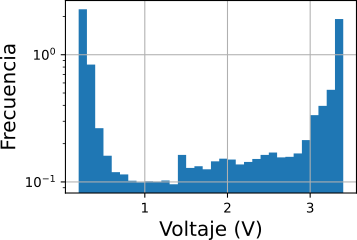
\includegraphics[width=0.5\textwidth]{histograma_puntos_pdf.png}
    \caption{\textbf{Histograma de voltajes} de una señal del PMT tomada con la RP a 31.25 MHz. El eje vertical está en escala logarítmica.}
    \label{fig:histograma_puntos}
\end{SCfigure}


\begin{figure}
    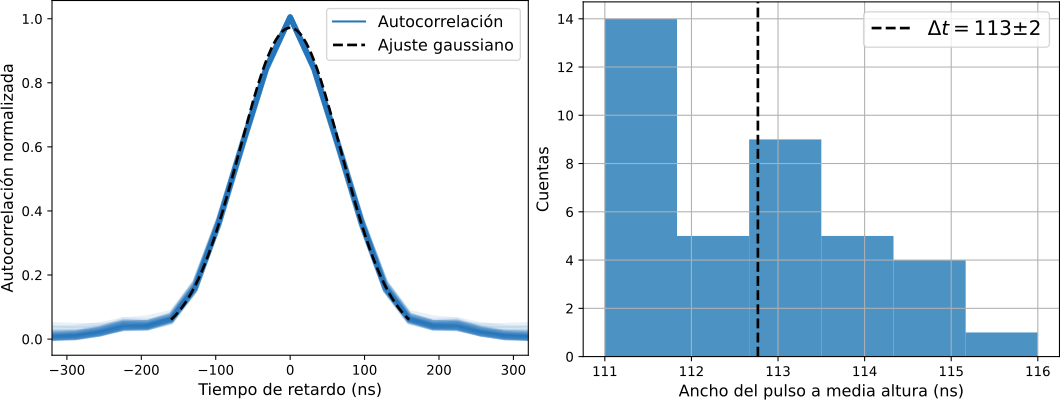
\includegraphics[width=\textwidth]{ancho_pulsos.png}
    \caption{\textbf{Autocorrelación} de las ventanas medidas por la RP a 31.25 MHz. A la izquierda se ve la autocorrelación de cada ventana y un ajuste gaussiano a una de ellas. A la derecha, un histograma de las desviaciones estandar de las gausianas.}
    \label{fig:ancho_pulsos}
\end{figure}

\subsection{Conteo de fotones} \label{sec:conteo}


Una vez que la RP obtiene la señal del PMT, el paso que queda para convertirla a intensidad lumínica es hacer un conteo de la cantidad de pulsos para la ventana de tiempo que midió.
Para esto, se necesita un algoritmo que tome como entrada la señal temporal del PMT $s(t)$, que muestreada es un conjunto discreto $\{s(t_i)\}$ y devuelva como salida el conjunto de tiempos $\{t_p\}$ en los que hay un pulso.
El algoritmo debe cumplir con dos condiciones: tiene que ser preciso para no sesgar los espectros y tiempos de vida, y tiene que ser rápido para que las mediciones se puedan hacer en tiempo real.

\begin{figure}
    \centering
    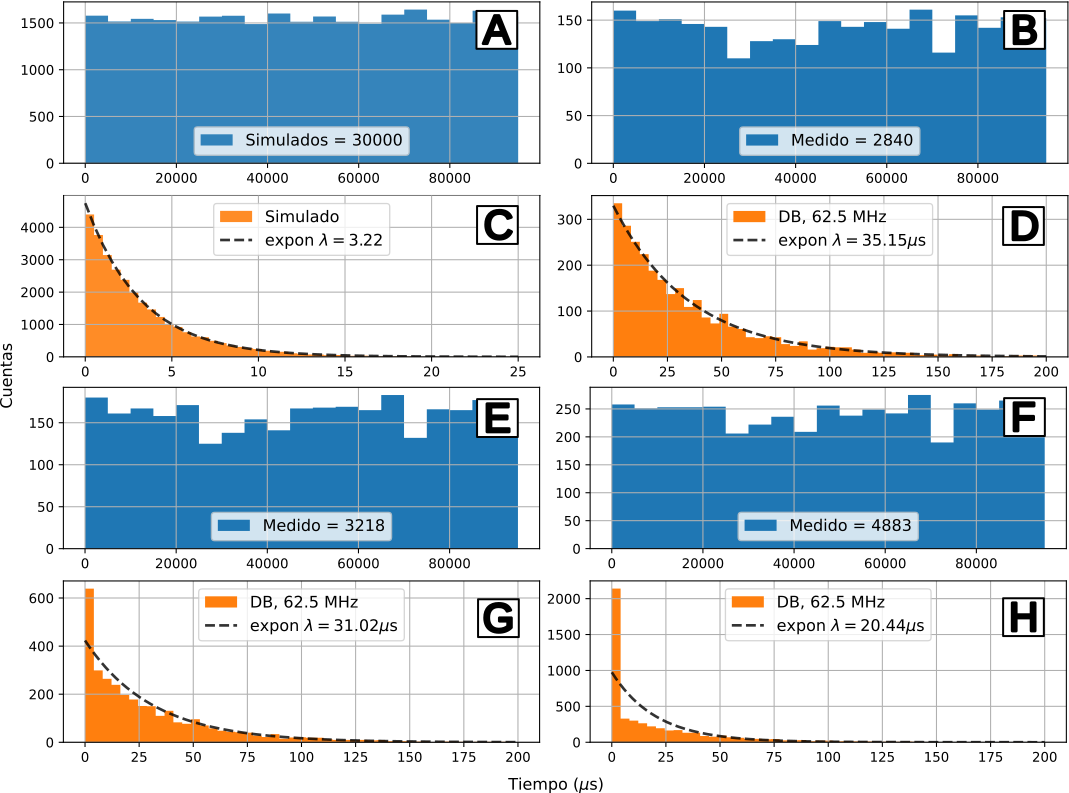
\includegraphics[width=\textwidth]{conteo.png}
    \caption{\textbf{Comparación de distintos métodos de conteo de fotones.} (\textbf{A}) distribución de pulsos simulados en un intervalo $T \sim 96$ ms y (\textbf{C}) distribución del tiempo $\Delta t$ entre esos pulsos. Análogamente, (\textbf{B}) y (\textbf{D}) para datos de pulsos medidos con frecuencia de muestreo de 31.25 MHz y detectados con el algoritmo $DB$. (\textbf{E}) y (\textbf{G}) medidos a 62.5 MHz y detectados con $DB$. (\textbf{F}) y (\textbf{H}) medidos a 31.25 MHz y detectados con $D$.}
    \label{fig:conteo}
\end{figure}

Nuestra implementación, que llamaremos DB, consiste en tres pasos, (i) binariza la señal temporal, (ii) busca los puntos en los que la derivada hace un salto y (iii) elimina los puntos que están muy cerca en el tiempo.
La binarización consiste en convertir en 1 a los puntos que sobrepasan (es decir, cuyo voltaje es menor que) cierto umbral $V_b$ y en 0 a los que no. 
Luego, se calcula la diferencia entre los puntos consecutivos $\Delta s(t_i) = s(t_{i+1}) - s(t_i)$, y se toma el conjunto $\{t_j\}$ en los que la diferencia es negativa.
Por último, se eliminan los puntos que estén a menos de $\Delta t_{min}$ de otros.
Si bien tanto $V_b$ como $\Delta t_{min}$ son configurables, los valores por defecto son $V_b = 1$V, que se tomó según lo encontrado en la sección \ref{sec:caracterizacion_pmt}, y $\Delta t_{min} = 0$, ya que vimos que cambiar este último valor no generaba una diferencia en los pulsos detectados.
Si bien existen otros algoritmos más sofisticados para encontrar picos, como la función \textit{find\_peaks\_cwt} o \textit{find\_peaks} del paquete de Python \textit{scipy}, estos suelen aplicar técnicas costosas computacionalmente, y por lo tanto lentas a comparación de tomar la derivada y binarización \cite{du_improved_2006}.

Una vez elegido el algoritmo, es necesario asegurarse que estuviera contando pulsos correctamente.
Para eso iluminamos una muestra con intensidad constante durante un intervalo $T$ de medición, calculamos la distribución de $\Delta t_j$ y la comparamos con una simulación equivalente para ganar intuición (\textbf{Fig. \ref{fig:conteo}}).
La diferencia $\Delta t_i = t_{i+1} - t_i$ entre dos variables aleatorias uniformemente distribuidas, y ordenadas de forma tal que $t_1 < ... < t_i < t_{i+1} < ... < t_N $ es otra variable aleatoria con distribución exponencial y valor medio $T/N$, donde $N$ es el número de pulsos detectados \cite{dasuniform}.
La simulación consiste en N = 30000 pulsos uniformemente distribuidos en un intervalo de $\sim 96$ ms, lo que da un valor medio de $\lambda \equiv \langle \Delta t_j \rangle = 3.22$ $\mu$s (\textbf{Fig. \ref{fig:conteo}A y C}).
Se tomó N = 30000 para tener una buena estadística a la hora de comparar con la distribución de probabilidad exacta (línea punteada en \textbf{Fig. \ref{fig:conteo}C}) con el mismo valor medio.
Realizamos la medición por el mismo intervalo de tiempo con una frecuencia de muestreo de 62.5 MHz al iluminar una muestra con CW.
El algoritmo \textit{DB} detectó 3218 pulsos, y se ve que la distribución de $\Delta t_j$ parece seguir una exponencial excepto por el primer intervalo del histograma que tiene un número de cuentas mucho mayor que el resto (\textbf{Fig. \ref{fig:conteo}E y G}).
Esto se debe a las fluctuaciones de alta frecuencia, que hacen que \textit{DB} detecte dos $t_j$ para un mismo pulso de la señal (ver \textbf{Fig. \ref{fig:pmt_signal}C}). 
Para resolver este problema se puede aumentar $\Delta t_{min}$ o reducir la frecuencia de muestreo.
La frecuencia de 31.25 MHz sigue siendo capaz de detectar pulsos (ver \ref{sec:caracterizacion_pmt}), por lo que realizamos el mismo análisis sub-muestreando la señal original.
En este caso \textit{DB} detectó 2840 pulsos, y se ve que la distribución de $\Delta t$ sigue una exponencial con valor medio $\lambda = 35.15 \mu$s (\textbf{Fig. \ref{fig:conteo}B y D}).
A modo de comparación, también procesamos la señal a 31.25 MHz, pero usando un algoritmo \textit{D} que consiste en tomar los puntos en los que la derivada es menor a un umbral (en este caso de -0.5).
Éste detectó 4883 pulsos, y se puede ver que también tiene el problema de detectar fluctuaciones de alta frecuencia, aumentando sintéticamente la cantidad de pulsos que hay en la señal (\textbf{Fig. \ref{fig:conteo}F y H}).

\begin{table}[t]
\centering
\begin{tabular}{|l|c|c|}
    \hline
    \textbf{Método} & \boldmath$\chi^2$ & \textbf{Tiempo (ms)} \\
    \hline
    DB 31.25 MHz & 47 & 9\\
    D 31.25 MHz & 2952 & 3\\
    DB 62.5 MHz & 230 & 9 \\
    \textit{find\_peaks} 31.25 MHz & 88 & 19 \\
    Crítico & 65 & - \\
    \hline
\end{tabular}
\caption{Comparación del estadístico $\chi^2$ y el tiempo de análisis para los distintos métodos. El tiempo de \textit{find\_peaks\_cwt} fue muy largo y no se agregó a la tabla.}
\label{tab:chisq}
\end{table}

Por último, para tener una medida cuantitativa de la bondad de ajuste al modelo exponencial, calculamos el $\chi^2$ dado por la fórmula 

\begin{equation}
    \chi^2  = \sum_{i=1}^{n=50} \frac{(O_i - E_i)^2}{E_i},
\end{equation}

\noindent donde $n$ es el número de barras en el histograma, $O_i$ es la cantidad de cuentas observadas, y $E_i$ es la cantidad de cuentas esperadas, asumiendo que la distribución de los datos debería ser una exponencial con el valor medio observado $\langle \Delta t \rangle$.
Obtuvimos los estadísticos de la tabla \ref{tab:chisq}, donde el $\chi^2$ crítico es el correspondiente a un test de hipótesis con significancia $\alpha = 0.05$ \cite{frodesen_probability_1979}.
Después de esta comparación entre algoritmos de detección y frecuencias de sampleo, concluimos que la elección óptima es tomar los datos a 31.25 MHz y usar el algoritmo de detección \textit{DB}.


